\documentclass[a4paper]{article}

\usepackage{xltxtra}
\XeTeXlinebreaklocale "th_TH" 
\XeTeXlinebreakpenalty = 100
\XeTeXlinebreakskip = 0pt plus 1pt
\linespread{1.5}
\setmainfont[
    Scale = MatchUppercase,
    Mapping = tex-text
]{TH Sarabun New}
\newfontfamily{\thaifont}[
    Scale = MatchUppercase,
    Mapping = tex-text
]{TH Sarabun New}

\renewcommand{\abstractname}{บทคัดย่อ}
\renewcommand{\figurename}{รูปที่}
\renewcommand{\tablename}{ตารางที่}
\renewcommand{\refname}{บรรณานุกรม}

\usepackage[
    top = 2.54cm,
    bottom = 2.54cm,
    left = 2.54cm,
    right = 2.54cm
]{geometry}

\graphicspath{{./images/}}

\usepackage[numbib]{tocbibind}
\usepackage[
    justification = centering,
    skip = 0pt
]{caption}
\usepackage{indentfirst}
\usepackage{pgfplots}
\pgfplotsset{compat = 1.18}
\usepackage{multirow}

\title{การศึกษาปัจจัยทางสังคมที่ส่งผลต่อจุดเวลาที่เริ่มใช้คำว่า “สาย”}
\author{
    ปานญุตม์ ศรีวิโรจน์\\6340138322
    \and
    วราลี วงษ์สมตระกูล\\6340209222
    \and
    สุชญา สุรพนานนชัย\\6340241222
    \and
    อภิมณฑ์ จิตรอักษร\\6340261822
}
\date{}

\begin{document}
\maketitle
\begin{abstract}
    คำบอกเวลาหลายคำเกี่ยวข้องกับกิจวัตรของมนุษย์และสามารถแสดงถึงการรับรู้ช่วงเวลาของบุคคลนั้นได้ เพราะช่วงเวลาของคำนั้นสามารถปรับเปลี่ยนไปได้ตามแต่ละบุคคล เช่น คำว่า “สาย” ที่มีความแตกต่างระหว่างบุคคลค่อนข้างมาก หรืออาจกล่าวได้ว่าแต่ละคนไม่ได้มีจุดเวลาที่เริ่มต้นใช้คำว่า “สาย” เป็นจุดเวลาเดียวกัน ซึ่งอาจเป็นผลมาจากปัจจัยทางด้านสังคมต่าง ๆ การศึกษานี้จึงมุ่งศึกษาความสัมพันธ์ของจุดเวลาที่เริ่มใช้คำว่า “สาย” กับปัจจัยทางสังคมต่าง ๆ อันประกอบด้วยปัจจัยด้านภูมิศาสตร์ อายุ และเพศ และดูความสัมพันธ์ระหว่างตัวแปรอายุและเพศควบคู่กันด้วย ผลการศึกษาพบว่าทั้งสามปัจจัยนี้ เมื่อแยกกัน ไม่มีปัจจัยใดที่ส่งผลต่อจุดเวลาที่เริ่มใช้คำว่า “สาย” อย่างมีนัยสำคัญอย่างสถิติ อย่างไรก็ตาม เมื่อศึกษาตัวแปรอายุและเพศควบคู่กัน กลับพบความแตกต่างระหว่างเพศที่มากกว่าในกลุ่มผู้ที่มีอายุมาก ในขณะที่กลุ่มที่มีอายุน้อยจะมีความแตกต่างจากปัจจัยเพศน้อยกว่า
\end{abstract}
\section{บทนำ}
    คำบอกเวลาเกี่ยวข้องกับกิจวัตรของมนุษย์อย่างชัดเจน และสะท้อนวิถีชีวิต วัฒนธรรมความเป็นอยู่ รวมถึงโลกทัศน์ของคนในแต่ละท้องถิ่นได้ พระยาอุปกิตศิลปสาร (2539, อ้างถึงในมิ่งมิตร ศรีประสิทธิ์, 2562) ได้จัดให้คำบอกเวลาอยู่ในหมวดคำวิเศษณ์ เรียกว่ากาลวิเศษณ์ ที่แสดงเวลาภายหน้าภายหลัง หรือเวลาปัจจุบัน หรือเวลาเร็ว ช้า ก่อน หลัง ฯลฯ

    น้อมนิจ วงศ์สุทธิธรรม (2515, อ้างถึงในมิ่งมิตร ศรีประสิทธิ์, 2562) พบว่าคำบอกเวลาในภาษาไทยมี 2 ประเภท\break หลัก ๆ คือ คำที่ทำหน้าที่เป็นหน่วยเสริมบอกเวลาตามลำพังได้ เช่น เช้า สาย ต่อไป ตะกี้ เที่ยง บ่าย ๆ เป็นต้น และคำบอกเวลาที่ทำหน้าที่เป็นหน่วยประโยคเสริมบอกเวลาตามลำพังไม่ได้ ต้องทำหน้าที่ร่วมกับคำบอกเวลาด้วยกันหรือร่วมกับคำในหมวดอื่น ๆ เช่น ครั้ง ชาติ ที่ เทอม ปี เป็นต้น

    นอกจากนี้แล้ว หากแบ่งคำบอกเวลาตามลำพังออกเป็นประเภทตามหน้าที่ของคำ ๆ นั้น ก็ยังสามารถแบ่งย่อยออกได้เป็น 3 ประเภทหลัก ๆ ได้แก่ คำบอกจุดของเวลาภายใน 1 วัน คำบอกวันเดือนปี และคำบอกระยะเวลา โดยคำบอกจุดเวลาภายใน 1 วัน จะสามารถแบ่งย่อยออกได้เป็นอีกหลายประเภท หนึ่งในนั้นคือคำบอกจุดของเวลาจากการสังเกตธรรมชาติและสิ่งแวดล้อมรอบตัว เช่น เช้า สาย เที่ยง บ่าย ซึ่งเป็นการบอกเวลาโดยกะประมาณ ไม่สามารถบอกเวลาที่เฉพาะเจาะจงเหมือนการใช้นาฬิกาได้ เนื่องจากเป็นคำบอกเวลาที่มีความสัมพันธ์ใกล้ชิดกับการสังเกต ทำให้แต่ละคนสามารถสังเกตลักษณะ\break ต่าง ๆ ได้ไม่เหมือนกัน (มิ่งมิตร ศรีประสิทธิ์, 2562)

    อย่างไรก็ตาม แม้คำบอกเวลาประเภทนี้จะสามารถปรับเปลี่ยนไปได้ตามแต่ละบุคคล ไม่ได้มีจุดเวลาที่ชัดเจน แต่จากการสังเกตและข้อมูลที่รวบรวมมาในเบื้องต้นกลับพบว่ามีบางคำที่จุดเวลาที่เริ่มต้นการใช้หลากหลายกว่าคำอื่น ๆ เช่น คำว่า “สาย” ซึ่งมีความแตกต่างระหว่างบุคคลค่อนข้างมาก กล่าวคือ แต่ละคนไม่ได้มองคำว่า “สาย” เป็นช่วงเวลาเดียวกัน เวลา 8 นาฬิกาอาจเป็นเวลาที่สายแล้วสำหรับบางคน ในขณะที่อีกคนอาจมองว่ายังไม่เริ่มเข้าสู่เวลาสายก็ได้ ต่างจากคำว่า "เช้า" ที่คนส่วนใหญ่มักจะเริ่มใช้พร้อมกันตอนหกนาฬิกา

    ด้วยเหตุนี้ ผู้ศึกษาจึงสนใจศึกษาความสัมพันธ์ของจุดเวลาที่เริ่มใช้คำว่า “สาย” กับปัจจัยทางสังคมต่าง ๆ อันได้แก่ ปัจจัยทางด้านภูมิศาสตร์ เนื่องจากคำว่า “สาย” เป็นหนึ่งในบอกเวลาที่เกี่ยวพันกับวิถีชีวิตและธรรมชาติของแต่ละพื้นที่ ผู้คนที่อาศัยอยู่ในพื้นที่ที่ต่างกันอาจมีจุดเวลาที่เริ่มใช้คำว่า “สาย” แตกต่างกันได้

    นอกจากนี้ ผู้ศึกษายังสนใจว่าจะยังมีปัจจัยอื่นที่ส่งผลต่อความแตกต่างที่เกิดขึ้นได้อีกหรือไม่ ซึ่งปัจจัยทางสังคมที่สำคัญและส่งผลต่อวิถีชีวิตของคน ๆ หนึ่งอย่างชัดเจน คือ อายุ และเพศ เนื่องจากบุคคลที่อาศัยอยู่พื้นที่เดียวกันแต่มีอายุต่างช่วงวัยกันอาจมีวิถีชีวิตที่ไม่เหมือนกัน ขึ้นอยู่กับภาระหน้าที่และความรับผิดชอบ ในขณะเดียวกัน วิถีชีวิตของคนที่อายุเท่ากันในแต่ละเพศก็อาจแตกต่างกันด้วยเช่นกัน ซึ่งอาจเป็นผลมาจากค่านิยมของสังคมบางอย่างที่หยั่งรากลึกอยู่ในสังคมไทย และเมื่อพิจารณาว่าค่านิยมดังกล่าวอาจเปลี่ยนไปตามยุคสมัย ผู้ศึกษาจึงเลือกศึกษาตัวแปรเพศและอายุควบคู่กันด้วย

    ตามนิยามของพจนานุกรม ฉบับราชบัณฑิตยสถาน พ.ศ. 2554 ได้ให้ความหมายคำว่า “สาย” ไว้ 2 ความหมาย นั่นคือ 1) เวลาระหว่างเช้ากับเที่ยง ประมาณ 9.00 น. ถึง 10.00 น. และ 2) ช้ากว่าที่กำหนด, ล่าช้า ในขณะที่การศึกษาของมิ่งมิตร ศรีประสิทธิ์ (2562) ได้ให้ความหมายของ “เวลาสาย” ไว้ว่าเป็นเวลาที่ดวงอาทิตย์ขึ้นสู่ท้องฟ้าแล้วส่องแสงยาวลงมา หรือส่องแสงสว่างจ้า ซึ่งนับเป็นคำบอกเวลาโดยการสังเกตดวงอาทิตย์เป็นหลัก ในการศึกษานี้ เราจะศึกษาเฉพาะคำว่า “สาย” ในความหมายแรกตามพจนานุกรม นั่นคือคำว่า “สาย” ที่ใช้ถึงการแสดงช่วงเวลาในหนึ่งวัน โดยไม่นับความหมายที่แปลว่าล่าช้ากว่ากำหนด เนื่องจากเป็นความหมายที่มีเวลาเทียบเคียงชัดเจนอยู่แล้ว จึงไม่ได้ทำให้เกิดความแตกต่างระหว่างบุคคลมากนัก
\section{ระเบียบวิธีวิจัย}
    เป้าหมายของการศึกษาครั้งนี้ คือทดสอบและพิสูจน์สมมติฐานทั้งหมด 4 ข้อ ได้แก่
    \begin{enumerate}
        \item คนที่อยู่ในอาศัยอยู่ในกรุงเทพ-ปริมณฑลจะเริ่มใช้คำว่า “สาย” เร็วกว่าคนที่ไม่ได้อาศัยอยู่ในกรุงเทพ-ปริมณฑล เนื่องจากผู้ศึกษามองว่าวิถีชีวิตของคนในเมืองหลวงมักจะต้องทำงานบริษัทที่มีเวลาเริ่มงานและเวลาเลิกงานที่ตายตัวชัดเจน และต้องใช้เวลาเดินทางมากกว่าในช่วงเวลาเร่งรีบ ซึ่งอาจะเป็นปัจจัยทำให้ต้องตื่นเช้าและเริ่มกิจวัตรเร็วกว่า ทำให้จุดเวลาที่ทำให้รู้สึกว่าสายเร็วกว่า
        \item คนที่อายุมากกว่าจะเริ่มใช้คำว่า “สาย” เร็วกว่าคนที่อายุน้อย เนื่องจากคนในสมัยก่อนเป็นรุ่นที่เติบโตมาโดยไม่มีโทรศัพท์หรือสัญญาณอินเตอร์เน็ต ทำให้ไม่ได้มีกิจกรรมให้ทำในเวลากลางคืนมากเท่าปัจจุบัน รวมถึงต้องตื่นมาทำงานในตอนเช้า ส่วนใหญ่จึงน่าจะติดนิสัยเข้านอนเร็วและตื่นเช้ากว่า ทำให้จุดที่เริ่มรู้สึกสายเร็วกว่า
        \item เพศหญิงจะเริ่มใช้คำว่า “สาย” เร็วกว่าเพศชาย เนื่องจากค่านิยมของสังคมที่คาดหวังให้ผู้หญิงตื่นเช้าหรือต้องตื่นมาทำอาหาร รวมถึงผู้หญิงอาจใช้เวลาในการเตรียมตัวหรือทำกิจวัตรนานกว่า ทำให้ต้องตื่นเช้ากว่าและเริ่มรู้สึกสายเร็วกว่า
        \item ความแตกต่างของจุดเวลาที่เริ่มใช้คำว่า “สาย” ระหว่างเพศชายและเพศหญิงจะชัดเจนกว่าในกลุ่มคนที่มีอายุมาก เนื่องจากค่านิยมในสมัยก่อนที่ผู้หญิงจะต้องตื่นเช้ามาทำอาหาร ในขณะที่กลุ่มคนที่มีอายุน้อยอาจไม่มีความแตกต่างนี้ เนื่องจากค่านิยมที่เปลี่ยนแปลงไป
    \end{enumerate}
\subsection{การเก็บข้อมูล}
    ในการเก็บข้อมูลเพื่อนำมาศึกษาความสัมพันธ์ระหว่างปัจจัยสังคมต่าง ๆ และการรับรู้ช่วงเวลา “สาย” ผู้ศึกษาจะใช้แบบสอบถามทางภาษา โดยในแบบสอบถามจะเก็บข้อมูลทั้งหมด 2 ส่วน ได้แก่ ข้อมูลพื้นฐาน และข้อมูลภาษา ดังนี้
    \begin{enumerate}
        \item ข้อมูลพื้นฐาน เป็นข้อมูลทั่วไปของผู้ตอบแบบสอบถามที่ผู้ศึกษาคาดว่าอาจเป็นตัวแปรที่นำมาศึกษาการรับรู้ช่วงเวลาของผู้ทำแบบสอบถามได้ ประกอบไปด้วย เพศ เชื้อชาติ อายุ การศึกษาขั้นสูงสุด เมือง อำเภอ หรือจังหวัดที่เติบโตและเมืองใหญ่ที่อยู่ใกล้สถานที่นั้น
        \item ข้อมูลภาษา เป็นข้อมูลจากการสอบถามว่าผู้ทำแบบสอบถามมองว่าแต่ละชั่วโมงจัดอยู่ในช่วงเวลาไหนของวัน เช่น เช้า สาย บ่าย เย็น ค่ำ ดึก เป็นต้น
    \end{enumerate}

    เพื่อให้ได้ข้อมูลที่เป็นระเบียบและง่ายต่อการนำมาศึกษา เมื่อได้ข้อมูลจากการทำแบบสอบถามเรียบร้อยแล้ว ผู้ศึกษาจะจัดเก็บข้อมูลที่ได้จากแบบถามลงในตาราง spread sheet โดยจัดเก็บให้อยู่ในรูปแบบที่กำหนดเพื่อให้ง่ายต่อการศึกษา ดังนี้
    \begin{enumerate}
        \item ผู้ศึกษาจะเก็บข้อมูลเพศ โดยกรอกเพศชายด้วยตัวอักษร “ช” และกรอกเพศหญิงด้วยตัวอักษร “ญ”
        \item กรอกข้อมูลเชื้อชาติแบบเต็ม เช่น ไทย ไทยจีน เป็นต้น
        \item กรอกอายุของผู้ทำแบบสอบถามด้วยเลขอารบิก
        \item แปลงการศึกษาขั้นสูงสุดให้อยู่ในรูปตัวเลข โดยนับจำนวนปีที่ศึกษาโดยไม่นับรวมชั้นอนุบาล เช่น ม.6 จะนับเป็น 12
        \item กรอกข้อมูลสถานที่เติบโตโดยใช้ข้อมูลเต็ม เช่น จังหวัดตรัง
        \item กรอกข้อมูลเมืองใหญ่โดยใช้ข้อมูลเต็ม เช่น พัทยา
        \item กรอกข้อมูลภาษาโดยใช้ตัวย่อตามที่กำหนด โดยหากคำตอบมีแค่คำเดียวให้กรอกตัวย่อของเวลาหรือช่วงเวลานั้นไปได้เลย เช่น สาย กรอกว่า “ส” แต่ถ้ามีมากกว่าหนึ่งคำตอบ ให้เขียนจำนวนคำตอบนำหน้าและกรอกตัวย่อของเวลาหรือช่วงเวลานั้น เช่น กรอกว่า 2(มืด,ดึก) เป็นต้น
    \end{enumerate}
\subsection{การวิเคราะห์ข้อมูล}
    เมื่อจัดเก็บข้อมูลเรียบร้อยแล้ว ผู้ศึกษาจะวิเคราะห์ความสัมพันธ์ระหว่างตัวแปรต้นและตัวแปรตาม โดยจัดกลุ่มปัจจัยทางสังคมที่คาดว่าอาจส่งผลต่อการรับรู้และการใช้คำว่า “สาย” ของผู้ทำแบบสอบถามเป็นตัวแปรต้น ได้แก่ ตัวแปรภูมิศาสตร์ ตัวแปรเพศ ตัวแปรอายุ ตัวแปรอายุและเพศ เนื่องจากเป็นปัจจัยทางสังคมที่มีแนวโน้มส่งผลกระทบต่อกิจวัตรประจำวันซึ่งอาจส่งผลต่อการการรับรู้ช่วงเวลาของผู้ทำแบบสอบถามได้ อ้างอิงตามคำถามวิจัยและสมมติฐานทั้ง 4 ข้อ

    ส่วนตัวแปรตาม กำหนดให้เป็นจุดเวลาที่เริ่มต้นใช้คำว่าสาย ซึ่งแบ่งออกเป็นสองกลุ่ม ได้แก่ ก่อน 10 นาฬิกาและ ตั้งแต่ 10 นาฬิกาเป็นต้นไป เนื่องจาความหมายของคำว่า “สาย” ตามพจนานุกรมหมายถึง เวลาระหว่างเช้ากับเที่ยง ประมาณ 9.00 น. ถึง 10.00 น. ซึ่งเวลา 9 นาฬิกาเป็นจุดเวลาที่อยู่ตรงกลางระหว่างเวลาเช้า คือ 6 นาฬิกา ถึง 12 นาฬิกาพอดี และหากบุคคลนั้นมองว่าเวลาสายเริ่มต้นหลัง 10 นาฬิกา หมายความว่าบุคคลนั้นมีจุดเวลาที่เริ่มใช้คำว่า “สาย” ช้ากว่าปกติ

    นอกจากนี้ จากการกระจายของจุดเวลาที่เริ่มใช้คำว่า “สาย” จะเห็นว่ามีจุดสูงสุดอยู่ที่เวลา 9 นาฬิกา การใช้จุดดังกล่าวเป็นจุดแบ่ง จะทำให้ตรวจจับการเบ้ที่แตกต่างกันของกลุ่มย่อยได้ง่าย
    \begin{figure}[!ht]
        \begin{center}
        \begin{tikzpicture}
        \begin{axis}[
            ybar, ymin = 0, nodes near coords,
            bar width = 1cm,
            symbolic x coords = {7, 8, 9, 10, 11},
            xtick distance = 1,
            enlarge x limits = 0.2,
            ylabel = {จำนวนผู้ที่เริ่มใช้คำว่าสาย (คน)},
            xlabel = {เวลา (นาฬิกา)}
        ]
            \addplot coordinates{
                (7,7)
                (8,38)
                (9,85)
                (10,54)
                (11,12)
            };
        \end{axis}
        \end{tikzpicture}
        \end{center}
        \caption{แผนภูมิแท่งแสดงจำนวนผู้ที่เริ่มใช้คำว่า “สาย” ณ เวลาต่าง ๆ}
    \end{figure}
    \newpage

    หลังจากจัดกลุ่มของตัวแปรต้นและตัวแปรตามแล้ว จะนำตัวแปรต้นมาหาความสัมพันธ์กับจุดเวลาที่เริ่มใช้คำว่า “สาย” โดยมีวิธีการ ดังนี้

    \textbf{คำถามวิจัยที่ 1 ตัวแปรภูมิศาสตร์ส่งผลให้จุดเวลาที่เริ่มใช้คำว่าสายแตกต่างกันหรือไม่}
    \begin{enumerate}
        \item ระบุตำแหน่งของจุดเวลาที่เริ่มใช้คำว่า “สาย” ตามกลุ่ม ก่อน 10 นาฬิกา และ ตั้งแต่ 10 นาฬิกาเป็นต้นไป ลงบนแผนที่ตามรหัสไปรษณีย์ของผู้ตอบแบบสอบถาม เพื่อดูการกระจายตัวของข้อมูล
        \item สร้างเส้นแบ่งเขตภาษาลงบนแผนที่เพื่อดูการเริ่มใช้คำว่า “สาย” ในแต่ละพื้นที่
        \item สร้างตารางข้อมูลเพื่อแสดงการกระจายตัวของการเริ่มใช้คำว่า “สาย” ในแต่ละพื้นที่ รวมทั้งคำนวณร้อยละของจำนวนผู้ตอบแบบสอบถามในพื้นที่นั้น
        \item นำข้อมูลไปหาค่าไคสแควร์และค่า p-value เพื่อทดสอบนัยสำคัญทางสถิติ
        \item สร้างแผนภูมิจากร้อยละที่คำนวณได้เพื่อเปรียบเทียบความแตกต่างการรับรู้ช่วงเวลา “สาย”
    \end{enumerate}

    \textbf{คำถามวิจัยที่ 2 ตัวแปรอายุส่งผลให้จุดเวลาที่เริ่มใช้คำว่าสายแตกต่างกันหรือไม่}
    \begin{enumerate}
        \item สร้างตารางข้อมูลเพื่อแสดงการกระจายตัวของการเริ่มใช้คำว่า “สาย” ในแต่ละช่วงอายุ รวมทั้งคำนวณร้อยละของจำนวนผู้ตอบแบบสอบถามในกลุ่มอายุนั้น
        \item นำข้อมูลไปหาไคสแควร์และค่า p-value เพื่อทดสอบนัยสำคัญทางสถิติ
        \item สร้างแผนภูมิจากร้อยละที่คำนวณได้เพื่อเปรียบเทียบความแตกต่างการรับรู้ช่วงเวลา “สาย”
    \end{enumerate}

    \textbf{คำถามวิจัยที่ 3 ตัวแปรเพศส่งผลให้จุดเวลาที่เริ่มใช้คำว่าสายแตกต่างกันหรือไม่}
    \begin{enumerate}
        \item สร้างตารางข้อมูลเพื่อแสดงการกระจายตัวของการเริ่มใช้คำว่า “สาย” ในแต่ละเพศ รวมทั้งคำนวณร้อยละของจำนวนผู้ตอบแบบสอบถามเพศนั้น ๆ
        \item นำข้อมูลไปหาไคสแควร์และค่า p-value เพื่อทดสอบนัยสำคัญทางสถิติ
        \item สร้างแผนภูมิจากร้อยละที่คำนวณได้เพื่อเปรียบเทียบความแตกต่างการรับรู้ช่วงเวลา “สาย”
    \end{enumerate}

    \textbf{คำถามวิจัยที่ 4 ตัวแปรอายุและตัวแปรเพศส่งผลให้จุดเวลาที่เริ่มใช้คำว่าสายแตกต่างกันหรือไม่}
    \begin{enumerate}
        \item สร้างตารางไขว้ เพื่อดูความสัมพันธ์ระหว่างสองตัวแปร คือ เพศและอายุ
        \item สร้างแผนภูมิจากตารางไขว้เพื่อเปรียบเทียบความแตกต่างการรับรู้ช่วงเวลา “สาย”
    \end{enumerate}
\section{ผลการศึกษา}
\subsection{ผลการศึกษาคำถามวิจัยที่ 1}
    แผนที่และเส้นแบ่งเขตภาษา (isogloss) แสดงให้เห็นกลุ่มคนที่เริ่มใช้คำว่า “สาย” ก่อน 10 นาฬิกา (หมุดสีเหลือง) และกลุ่มคนที่เริ่มใช้คำว่า “สาย” ตั้งแต่ 10 นาฬิกาเป็นต้นไป (หมุดสีน้ำเงิน) บนแผนที่ประเทศไทย
    \begin{figure}[!ht]
        \begin{center}
        \begin{minipage}{0.45\textwidth}
            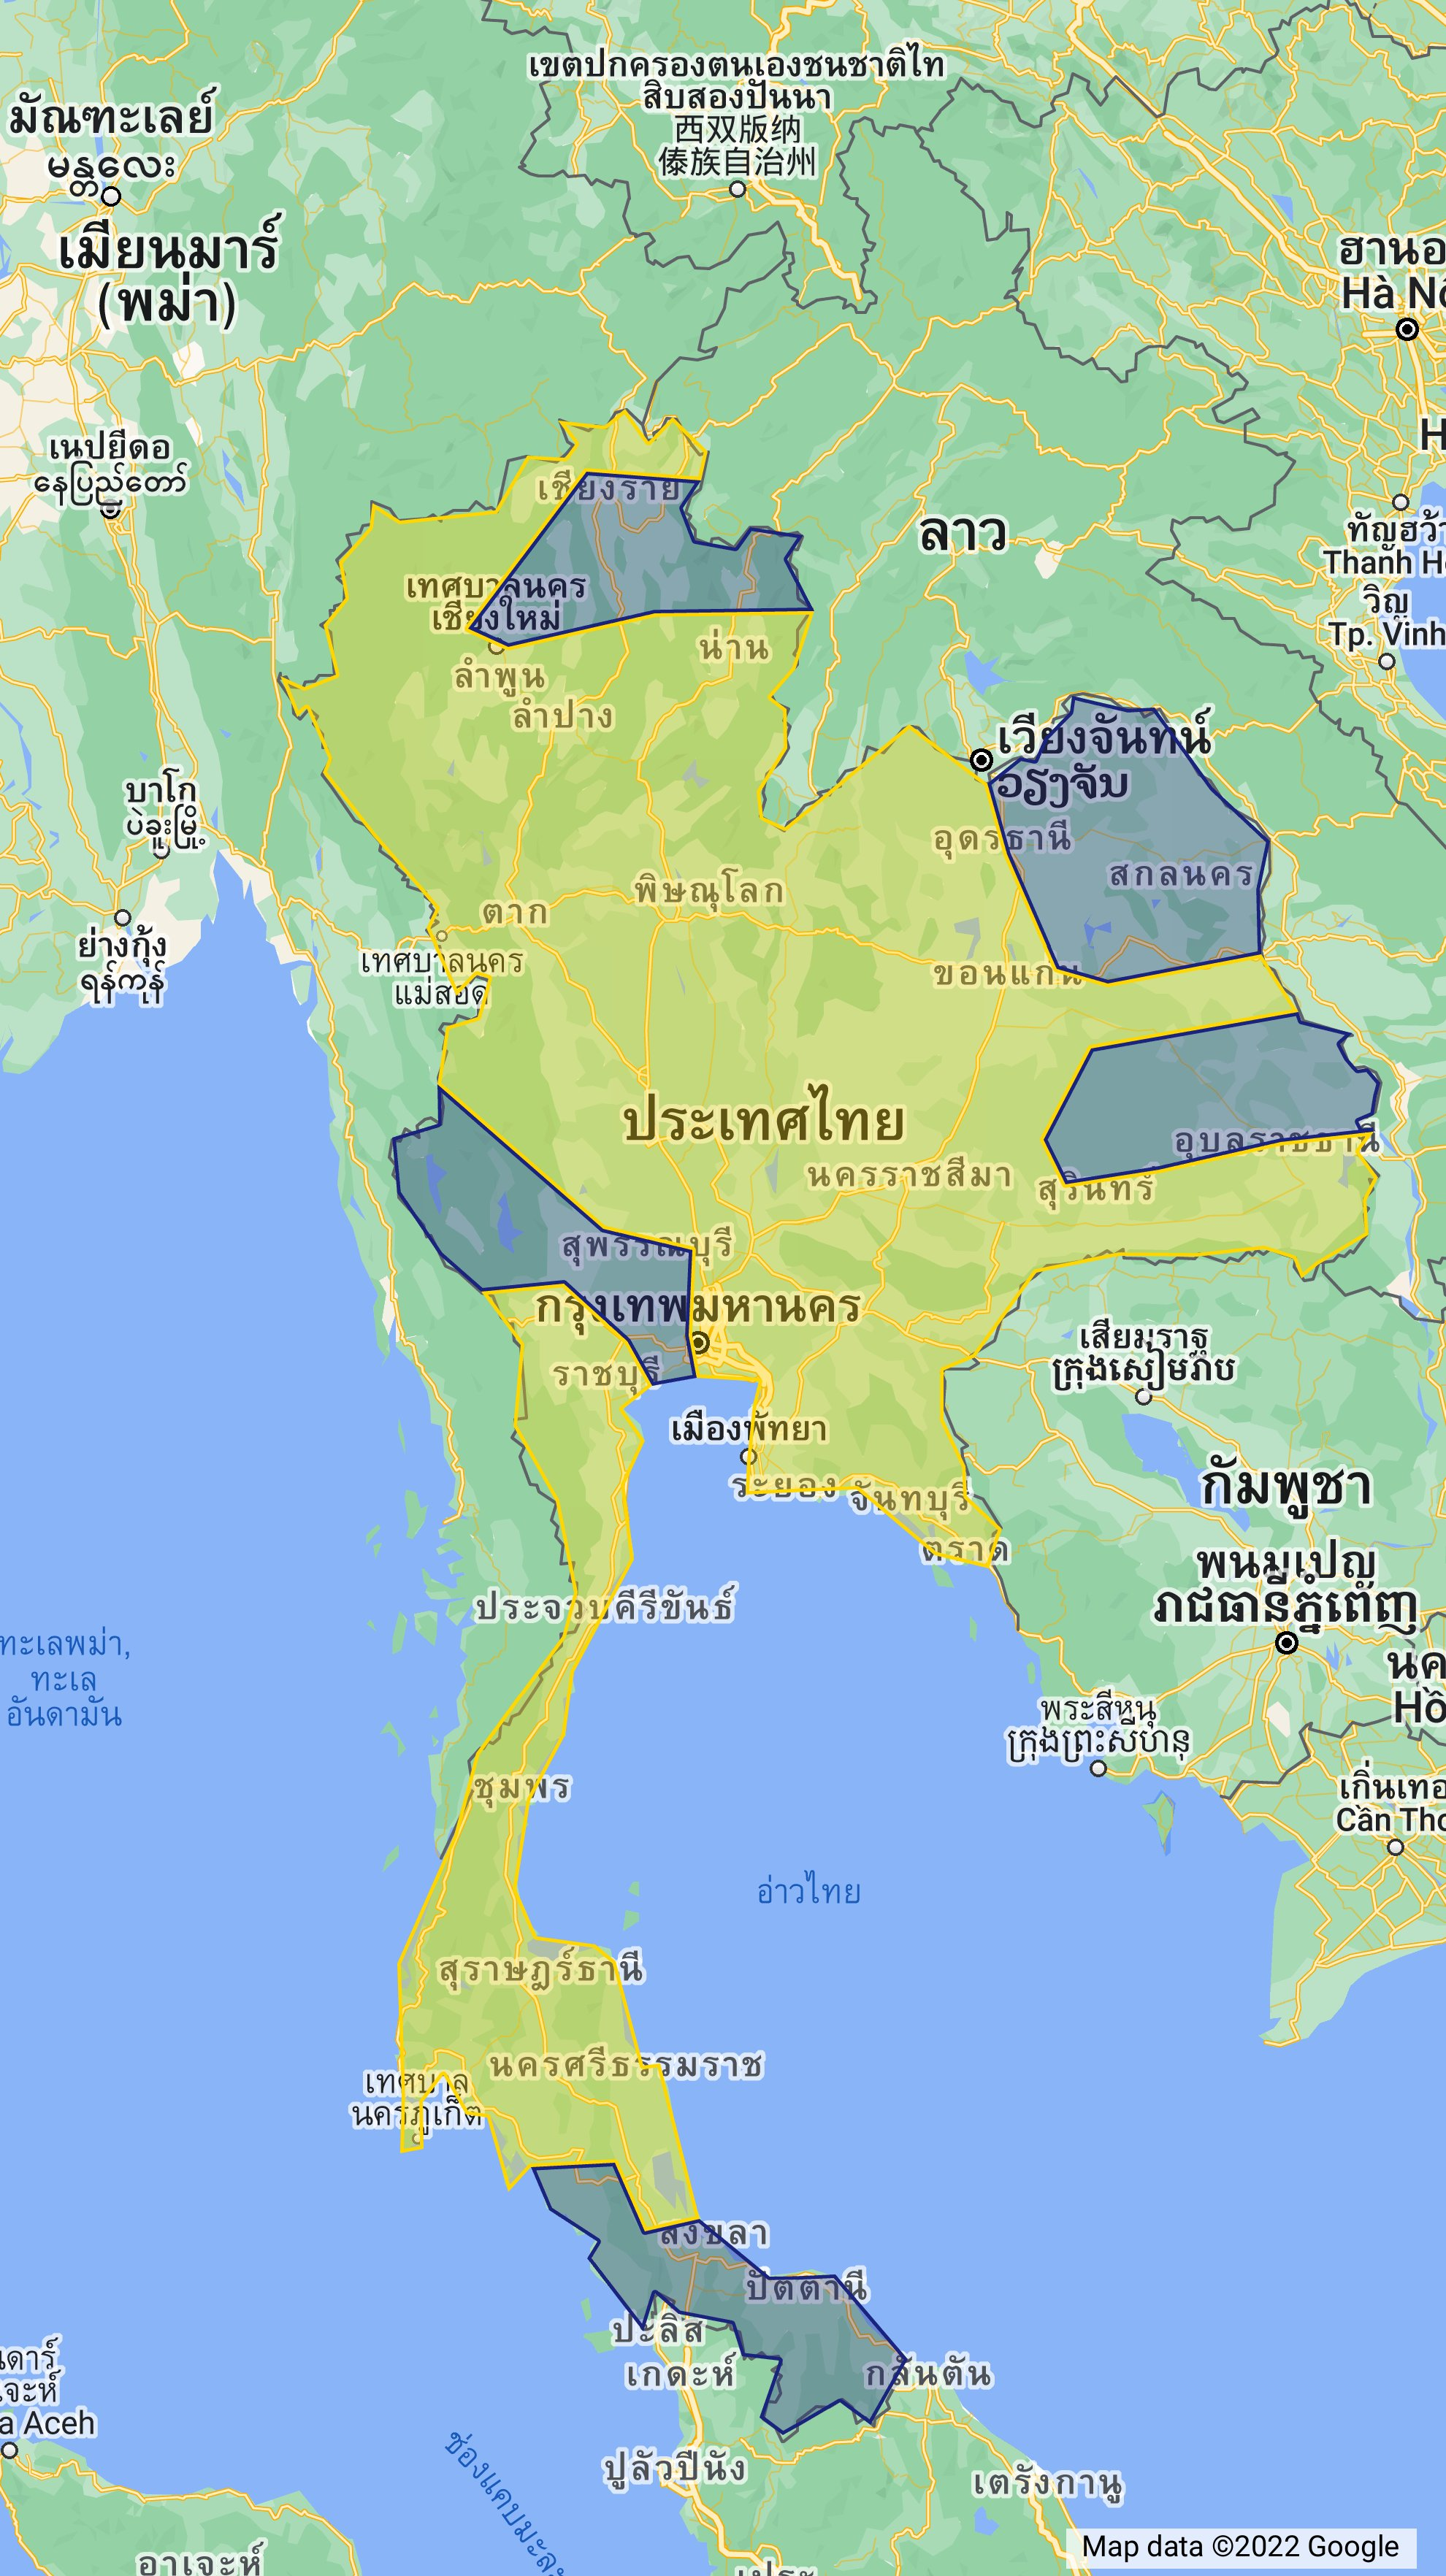
\includegraphics[width=0.9\textwidth]{map_no_dot}
        \end{minipage}
        \begin{minipage}{0.45\textwidth}
            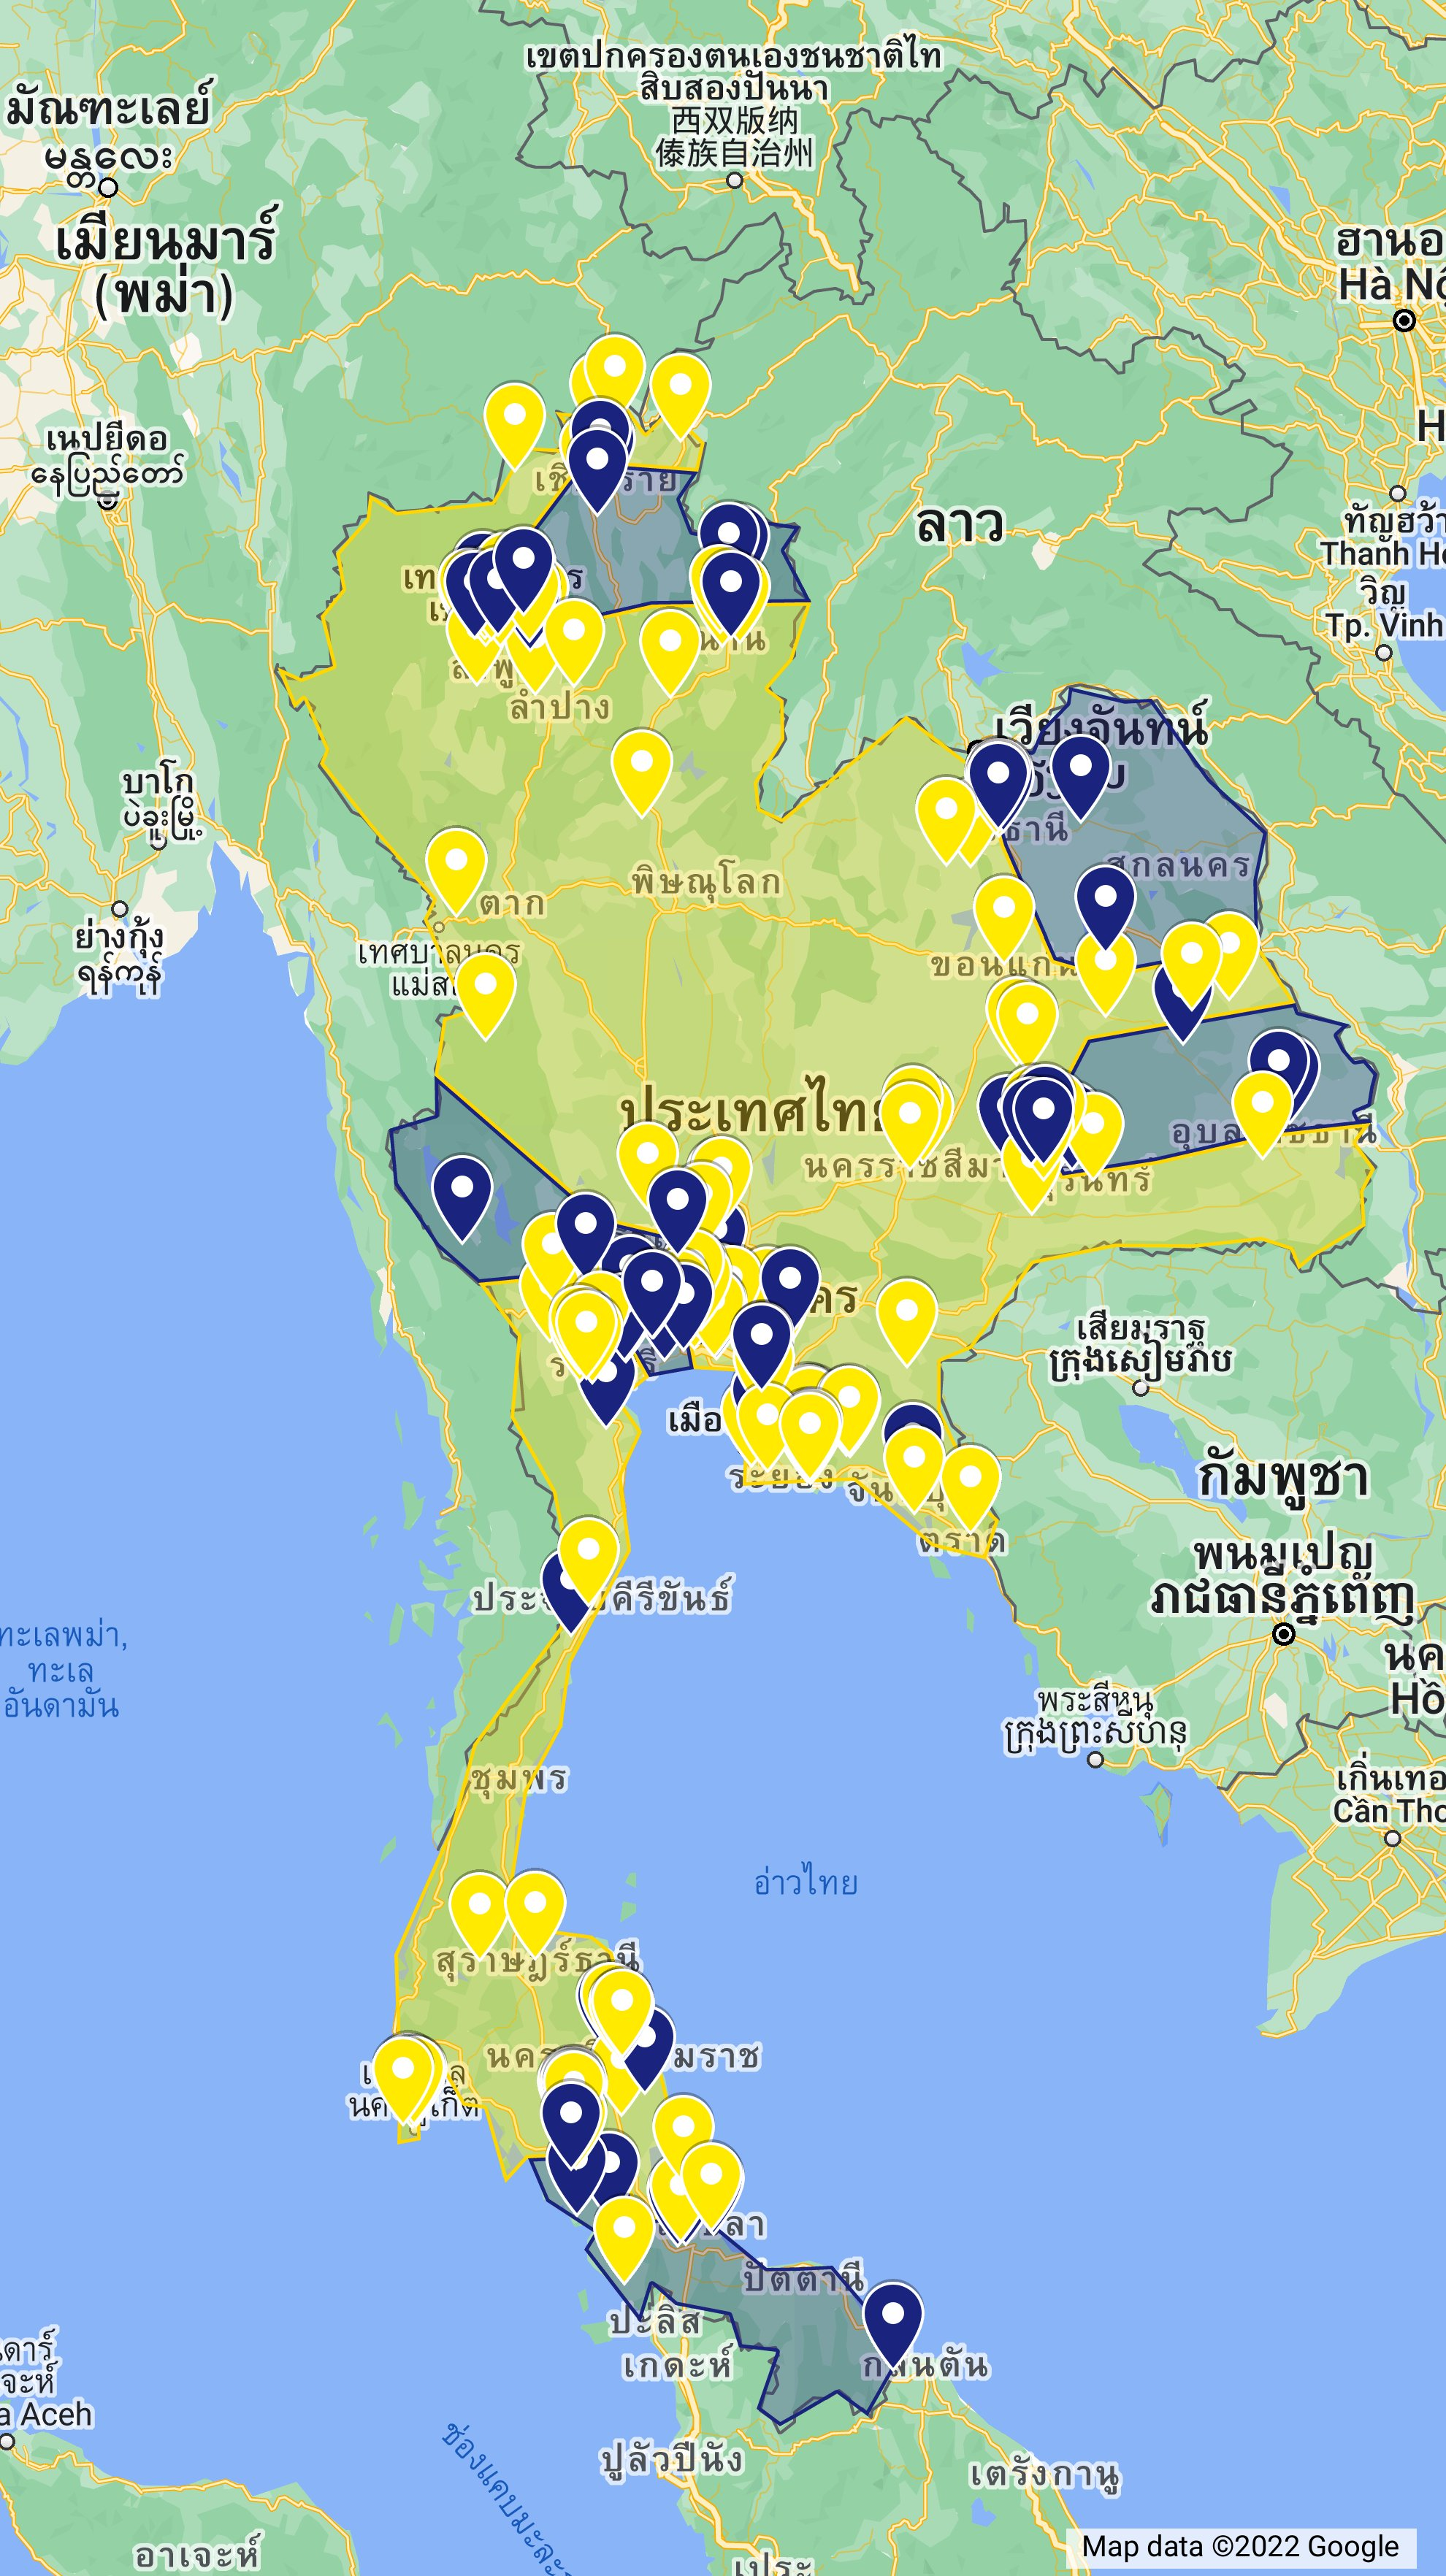
\includegraphics[width=0.9\textwidth]{map_with_dot}
        \end{minipage}
        \end{center}
        \caption{แผนที่แสดงเส้นแบ่งเขตภาษาของจุดเวลาที่เริ่มใช้คำว่า “สาย”}
    \end{figure}

    และจากการทำตารางไขว้ (Cross tabulation table) ระหว่างตัวแปรจังหวัดที่เติบโตและจุดเวลาที่เริ่มที่เริ่มใช้คำว่า “สาย” เพื่อทดสอบไคสแควร์ (Chi-squared Test) ได้ค่า $\chi^2$ = 0.0283 และค่า p-value = 0.867 ซึ่งมากกว่า 0.05 แสดงว่าตัวแปรทั้งสองไม่มีความสัมพันธ์กันอย่างมีนัยสำคัญทางสถิติ จึงปฏิเสธสมมติฐานที่ 1 ที่ตั้งไว้ว่าคนที่อยู่ในอาศัยอยู่ในกรุงเทพ-ปริมณฑลจะเริ่มใช้คำว่า “สาย” เร็วกว่าคนที่ไม่ได้อาศัยอยู่ในกรุงเทพ-ปริมณฑล
    \begin{table}[!ht]
        \begin{center}
        \begin{tabular}{|c|c|c|c|c|}
            \cline{3-5}
            \multicolumn{2}{c|}{} & \multicolumn{2}{c|}{จุดเวลาที่เริ่มใช้คำว่า “สาย”} & \multirow{2}{*}{รวม} \\
            \cline{3-4}
            \multicolumn{2}{c|}{} & ก่อน 10 น. & 10 น. เป็นต้นไป & \\
            \hline
            \multirow{2}{*}{จังหวัดที่เติบโต} & กรุงเทพและปริมณฑล & 20 & 10 & 30 \\
            \cline{2-5}
            & ไม่ใช่กรุงเทพและปริมณฑล & 110 & 59 & 169 \\
            \hline
            \multicolumn{2}{|c|}{รวม} & 130 & 69 & 199 \\
            \hline
        \end{tabular}
        \end{center}
        \caption{ตารางไขว้ระหว่างจังหวัดที่เติบโตและจุดเวลาที่เริ่มใช้คำว่า “สาย”}
    \end{table}
    \begin{figure}[!ht]
        \begin{center}
        \begin{tikzpicture}
        \begin{axis}[
            ybar, ymin = 0, ymax = 100,
            bar width = 1cm, nodes near coords,
            xtick distance = 1,
            enlarge x limits = 0.5,
            symbolic x coords = {กรุงเทพและปริมณฑล, ไม่ใช่กรุงเทพและปริมณฑล},
            xlabel = {จังหวัดที่เติบโต},
            ylabel = {ร้อยละของผู้ที่เริ่มใช้คำว่า “สาย” ก่อน 10 น.}
        ]
            \addplot coordinates{
                (กรุงเทพและปริมณฑล,66.66666667)
                (ไม่ใช่กรุงเทพและปริมณฑล,65.0887574)
            };
        \end{axis}
        \end{tikzpicture}
        \end{center}
        \caption{แผนภูมิแท่งแสดงร้อยละของผู้ที่เริ่มใช้คำว่า “สาย” ก่อน 10 น. แบ่งตามจังหวัดที่เติบโต}
    \end{figure}
\subsection{ผลการศึกษาคำถามวิจัยที่ 2}
    จากการทำตารางไขว้ (Cross tabulation table) ระหว่างตัวแปรช่วงวัยและจุดเวลาที่เริ่มใช้คำว่า “สาย” เพื่อทดสอบไคสแควร์ (Chi-squared Test) ได้ค่า $\chi^2$ = 0.665 และค่า p-value = 0.717 ซึ่งมากกว่า 0.05 แสดงว่าตัวแปรทั้งสองไม่มีความสัมพันธ์กันอย่างมีนัยสำคัญทางสถิติ จึงปฏิเสธสมมติฐานที่ 2 ที่ตั้งไว้ว่าคนที่อายุมากกว่าจะเริ่มใช้คำว่า “สาย” เร็วกว่าคนที่อายุน้อย
    \begin{table}[!ht]
        \begin{center}
        \begin{tabular}{|c|c|c|c|c|}
            \cline{3-5}
            \multicolumn{2}{c|}{} & \multicolumn{2}{c|}{จุดเวลาที่เริ่มใช้คำว่า “สาย”} & \multirow{2}{*}{รวม} \\
            \cline{3-4}
            \multicolumn{2}{c|}{} & ก่อน 10 น. & 10 น. เป็นต้นไป & \\
            \hline
            \multirow{3}{*}{ช่วงวัย} & วัยเรียน & 32 & 19 & 51 \\
            \cline{2-5}
            & วัยทำงาน & 88 & 43 & 131 \\
            \cline{2-5}
            & วัยเกษียณ & 10 & 7 & 17 \\
            \hline
            \multicolumn{2}{|c|}{รวม} & 130 & 69 & 199 \\
            \hline
        \end{tabular}
        \end{center}
        \caption{ตารางไขว้ระหว่างช่วงวัยและจุดเวลาที่เริ่มใช้คำว่า “สาย”}
    \end{table}
    \begin{figure}[!ht]
        \begin{center}
        \begin{tikzpicture}
        \begin{axis}[
            ybar, ymin = 0, ymax = 100,
            bar width = 1cm, nodes near coords,
            xtick distance = 1,
            enlarge x limits = 0.4,
            symbolic x coords = {วัยเรียน, วัยทำงาน, วัยเกษียณ},
            xlabel = {ช่วงวัย},
            ylabel = {ร้อยละของผู้ที่เริ่มใช้คำว่า “สาย” ก่อน 10 น.}
        ]
            \addplot coordinates{
                (วัยเรียน,62.74509804)
                (วัยทำงาน,67.17557252)
                (วัยเกษียณ,58.82352941)
            };
        \end{axis}
        \end{tikzpicture}
        \end{center}
        \caption{แผนภูมิแท่งแสดงร้อยละของผู้ที่เริ่มใช้คำว่า “สาย” ก่อน 10 น. แบ่งตามช่วงวัย}
    \end{figure}
\subsection{ผลการศึกษาคำถามวิจัยที่ 3}
    จากการทำตารางไขว้ (Cross tabulation table) ระหว่างตัวแปรเพศและจุดเวลาที่เริ่มใช้คำว่า “สาย” เพื่อทดสอบ\break ไคสแควร์ (Chi-squared Test) ได้ค่า $\chi^2$ = 2.008 และค่า p-value = 0.156 ซึ่งมากกว่า 0.05 แสดงว่าตัวแปรทั้งสองไม่มีความสัมพันธ์กันอย่างมีนัยสำคัญทางสถิติ จึงปฏิเสธสมมติฐานที่ 3 ที่ตั้งไว้ว่าเพศหญิงจะเริ่มใช้คำว่า “สาย” เร็วกว่าเพศชาย
    \begin{table}[!ht]
        \begin{center}
        \begin{tabular}{|c|c|c|c|c|}
            \cline{3-5}
            \multicolumn{2}{c|}{} & \multicolumn{2}{c|}{จุดเวลาที่เริ่มใช้คำว่า “สาย”} & \multirow{2}{*}{รวม} \\
            \cline{3-4}
            \multicolumn{2}{c|}{} & ก่อน 10 น. & 10 น. เป็นต้นไป & \\
            \hline
            \multirow{2}{*}{เพศ} & หญิง & 92 & 42 & 134 \\
            \cline{2-5}
            & ชาย & 38 & 27 & 65 \\
            \hline
            \multicolumn{2}{|c|}{รวม} & 130 & 69 & 199 \\
            \hline
        \end{tabular}
        \end{center}
        \caption{ตารางไขว้ระหว่างเพศและจุดเวลาที่เริ่มใช้คำว่า “สาย”}
    \end{table}
    \begin{figure}[!ht]
        \begin{center}
        \begin{tikzpicture}
        \begin{axis}[
            ybar, ymin = 0, ymax = 100,
            bar width = 1cm, nodes near coords,
            xtick distance = 1,
            enlarge x limits = 0.7,
            symbolic x coords = {หญิง, ชาย},
            xlabel = {เพศ},
            ylabel = {ร้อยละของผู้ที่เริ่มใช้คำว่า “สาย” ก่อน 10 น.}
        ]
            \addplot coordinates{
                (หญิง,68.65671642)
                (ชาย,58.46153846)
            };
        \end{axis}
        \end{tikzpicture}
        \end{center}
        \caption{แผนภูมิแท่งแสดงร้อยละของผู้ที่เริ่มใช้คำว่า “สาย” ก่อน 10 น. แบ่งตามเพศ}
    \end{figure}
    \newpage
\subsection{ผลการศึกษาคำถามวิจัยที่ 4}
    จากการทำตารางไขว้ (Cross tabulation table) ระหว่างตัวแปรช่วงวัยและเพศ พบว่าช่วงวัยที่เห็นความแตกต่างระหว่างเพศชัดที่สุดคือวัยเกษียณ โดยมีค่าร้อยละของผู้ที่เริ่มใช้คำว่า “สาย” ก่อน 10 นาฬิกาในเพศหญิงอยู่ที่ 77.78\% และในเพศชายอยู่ที่ 37.50\% ช่วงวัยที่เห็นความแตกต่างชัดรองลงมาคือวัยเรียนโดยมีค่าร้อยละของผู้ที่เริ่มใช้คำว่า “สาย” ก่อน 10 นาฬิกาในเพศหญิงอยู่ที่ 66.67\% และในเพศชายอยู่ที่ 55.56\% และช่วงวัยที่เห็นความแตกต่างน้อยที่สุดคือวัยทำงาน โดยมีค่าร้อยละของผู้ที่เริ่มใช้คำว่า “สาย” ก่อน 10 นาฬิกาในเพศหญิงอยู่ที่ 68.48\% และในเพศชายอยู่ที่ 64.10\%
    \begin{table}[!ht]
        \begin{center}
        \begin{tabular}{|c|c|c|c|}
            \cline{3-4}
            \multicolumn{2}{c|}{} & \multicolumn{2}{c|}{เพศ} \\
            \cline{3-4}
            \multicolumn{2}{c|}{} & หญิง & ชาย \\
            \hline
            \multirow{3}{*}{ช่วงวัย} & วัยเรียน & 22/33 (66.67\%) & 10/18 (55.56\%) \\
            \cline{2-4}
            & วัยทำงาน & 63/92 (68.48\%) & 25/39 (64.1\%) \\
            \cline{2-4}
            & วัยเกษียณ & 7/9 (77.78\%) & 3/8 (37.5\%) \\
            \hline
        \end{tabular}
        \end{center}
        \caption{ตารางแสดงอัตราส่วนและร้อยละของผู้ที่เริ่มใช้คำว่า “สาย” ก่อน 10 น. แบ่งตามเพศและช่วงวัย}
    \end{table}
    \begin{figure}[!ht]
        \begin{center}
        \begin{tikzpicture}
        \begin{axis}[
            ybar, ymin = 0, ymax = 100,
            bar width = 0.5cm, nodes near coords,
            symbolic x coords = {วัยเรียน, วัยทำงาน, วัยเกษียณ},
            xtick distance = 1,
            enlarge x limits = 0.4,
            xlabel = {ช่วงวัย},
            ylabel = {ร้อยละของผู้ที่เริ่มใช้คำว่า “สาย” ก่อน 10 น.},
            legend pos = outer north east
        ]
            \addplot coordinates{
                (วัยเรียน,66.66666667)
                (วัยทำงาน,68.47826087)
                (วัยเกษียณ,77.77777778)
            };
            \addlegendentry{เพศหญิง};
            \addplot coordinates{
                (วัยเรียน,55.55555556)
                (วัยทำงาน,64.1025641)
                (วัยเกษียณ,37.5)
            };
            \addlegendentry{เพศชาย};
        \end{axis}
        \end{tikzpicture}
        \end{center}
        \caption{แผนภูมิแท่งแสดงร้อยละของผู้ที่เริ่มใช้คำว่า “สาย” ก่อน 10 น. แบ่งตามเพศและช่วงวัย}
    \end{figure}
    \newpage
\section{อภิปรายผล}
\subsection{อภิปรายผลการศึกษาคำถามวิจัยที่ 1}
    จากแผนที่และเส้นแบ่งเขตภาษา จะเห็นได้ว่ากลุ่มคนที่เริ่มใช้คำว่า “สาย” ก่อน 10 นาฬิกา และกลุ่มคนที่เริ่มใช้คำว่า “สาย” ตั้งแต่ 10 นาฬิกาเป็นต้นไป มีการกระจายตัวที่ค่อนข้างกระจัดกระจายทั่วประเทศ ไม่ได้อยู่กันเป็นกลุ่มก้อนชัดเจนเป็นจังหวัดหรือเป็นภูมิภาค และในบริเวณกรุงเทพและปริมณฑลก็ไม่พบกลุ่มคนที่เริ่มใช้คำว่าสายเร็วกว่าสิบนาฬิกามากนัก หรืออาจกล่าวได้ว่าการอาศัยอยู่ในกรุงเทพและปริมณฑลหรือการอยู่ใกล้กับเมืองใหญ่ไม่ได้มีความสัมพันธ์กับจุดเวลาที่เริ่มใช้คำว่าสายอย่างมีนัยสำคัญ ซึ่งไม่สอดคล้องกับสมมติฐานที่ตั้งไว้ในตอนแรก ทั้งนี้ อาจมีปัจจัยอื่นที่ส่งผลต่อการรวมกลุ่ม\break เล็ก ๆ ในแต่ละส่วน เช่น อาชีพของคนในกลุ่มนั้น แหล่งท่องเที่ยวในเวลากลางคืน ซึ่งไม่สามารถสรุปได้เนื่องจากไม่มีข้อมูลมากพอ แต่อาจเป็นประเด็นในการศึกษาต่อไปในอนาคตได้
\subsection{อภิปรายผลการศึกษาคำถามวิจัยที่ 2}
    ข้อมูลจากตารางแสดงและกราฟให้เห็นว่า ผู้ทำแบบสอบถามในแต่ละช่วงอายุ ไม่ได้มีความแตกต่างอย่างมีนัยสำคัญในการใช้คำว่า “สาย” เมื่อเทียบระหว่างคนที่เริ่มใช้ในจุดเวลาก่อน 10 นาฬิกาและตั้งแต่ 10 นาฬิกา เนื่องจากค่าร้อยละในกราฟ แสดงสัดส่วนการใช้คำว่า “สาย” ของแต่ละช่วงวัยที่ไม่ต่างกันมากนัก นอกจากนี้ เมื่อทดสอบค่า p-value แล้วพบว่าตัวแปรทั้งสองไม่ได้มีความสัมพันธ์กันอย่างมีนัยสำคัญ หรืออาจกล่าวได้ว่า อายุไม่ใช่ตัวแปรสำคัญในการแปรของจุดเวลาที่เริ่มใช้คำว่า “สาย” ซึ่งไม่สอดคล้องกับสมมติฐานที่ตั้งไว้
\subsection{อภิปรายผลการศึกษาคำถามวิจัยที่ 3}
    จากข้อมูลจะเห็นได้ว่าเมื่อวัดเป็นค่าร้อยละแล้ว เพศชายและเพศหญิงเริ่มใช้คำว่า “สาย” ก่อน 10 นาฬิกาในสัดส่วนที่ใกล้เคียงกัน ไม่ได้มีความแตกต่างกันอย่างชัดเจน และเมื่อทดสอบค่า p-value แล้วก็พบว่าตัวแปรทั้งสองไม่ได้มีความสัมพันธ์กันอย่างมีนัยสำคัญ หรืออาจกล่าวได้ว่า เพศไม่ใช่ปัจจัยสำคัญในการเริ่มรับรู้เวลาสาย ซึ่งไม่สอดคล้องกับสมมติฐานที่ตั้งไว้ในตอนแรก
\subsection{อภิปรายผลการศึกษาคำถามวิจัยที่ 4}
    ผลจากการวิเคราะห์ Cross-tabulation และแผนภูมิแท่งแสดงให้เห็นว่าความแตกต่างของจุดเวลาที่เริ่มใช้คำว่า “สาย” ระหว่างเพศชายและเพศหญิงจะชัดเจนที่สุดในวัยเกษียณตรงกับกับข้อสันนิษฐานที่ตั้งไว้ว่า ความแตกต่างของจุดเวลาที่เริ่มใช้คำว่า “สาย” ระหว่างเพศชายและเพศหญิงจะชัดเจนกว่าในกลุ่มคนที่มีอายุมาก นอกจากนี้ยังสามารถวิเคราะห์ความสัมพันธ์ระหว่างช่วงวัยต่าง ๆ กับเพศได้ว่าสัดส่วนของผู้ที่เริ่มใช้คำว่า “สาย” ก่อนเวลา 10 นาฬิกาจะมีแนวโน้มมากขึ้น\break เรื่อย ๆ ในเพศหญิง โดยมีค่าร้อยละเรียงจากวัยเรียนสู่วัยเกษียณอยู่ที่ 66.67\%, 68.48\% และ 77.78\% ตามลำดับ จึงกล่าวได้ว่ามีแนวโน้มที่ผู้หญิงที่อายุมากขึ้นจะเริ่มใช้คำว่า “สาย” ก่อน 10 นาฬิกามากขึ้น อย่างไรก็ตามไม่พบความสัมพันธ์กันระหว่างช่วงวัยและการเริ่มใช้คำว่า “สาย” ก่อน 10 นาฬิกาในเพศชาย
\section{สรุป}
    จากคำถามวิจัยทั้ง 4 ข้อ จะเห็นได้ว่าไม่มีตัวแปรใดที่ส่งผลต่อจุดเวลาที่เริ่มใช้คำว่า “สาย” อย่างมีนัยสำคัญ ไม่ว่าจะเป็นปัจจัยทางภูมิศาสตร์ อายุ หรือเพศ อย่างไรก็ตาม เมื่อพิจารณาตัวแปรเพศควบคู่กับช่วงวัยแล้ว จะสังเกตเห็นความ\break แตกต่างระหว่างเพศที่ไม่เท่ากันในแต่ละช่วงวัย ซึ่งเป็นประเด็นที่อาจนำไปศึกษาต่อได้ในอนาคต ทั้งนี้ อาจเป็นเพราะข้อมูลที่รวบรวมมามีจำนวนน้อยเกินไป และมีการกระจายตัวในแต่ละกลุ่มที่ไม่เท่ากัน เช่น กลุ่มตัวอย่างในวัยเกษียณมีน้อย หรือเพศหญิงมีจำนวนมากกว่าเพศชาย รวมถึงอาจมีตัวแปรอื่น ๆ ที่ส่งผลต่อจุดเวลาที่เริ่มใช้คำว่า “สาย” เช่น อาชีพ แต่เป็นข้อมูลที่ ไม่ได้เก็บรวบรวมมาจากผู้ตอบแบบสอบถาม จึงเป็นประเด็นที่น่าสนใจเช่นกัน
\begin{thebibliography}{9}
    \bibitem{dictionary} พจนานุกรม ฉบับราชบัณฑิตยสถาน. (2554). สาย. สืบค้นจาก https://dictionary.orst.go.th
    \bibitem{mingmit} มิ่งมิตร ศรีประสิทธิ์. (2562). คำบอกเวลาในภาษาไทยถิ่นกลาง. \textit{วรรณวิทัศน์, 19}(2), 104–141. DOI:10.14456/vannavidas.2019.13
\end{thebibliography}
\end{document}